\documentclass{beamer}
\mode<presentation>
\usetheme{CambridgeUS}
\usepackage[russian]{babel}
\usepackage[utf8]{inputenc}
\usepackage[T2A]{fontenc}
\usepackage{sansmathaccent}

\usepackage{verbatim}
\usepackage{alltt}

\pdfmapfile{+sansmathaccent.map}
\title[Язык C]{Буферизованный ввод-вывод, часть 5}
\author{Наумов Д.А., доц. каф. КТ}
\date[25.09.2019] {Операционные системы и системное программное обеспечение, 2019}

\begin{document}

%ТИТУЛЬНЫЙ СЛАЙД
\begin{frame}
  \titlepage
\end{frame}
  
%СОДЕРЖАНИЕ ЛЕКЦИИ
\begin{frame}
  \frametitle{Содержание лекции}
  \tableofcontents  
\end{frame}

\section{Буферизованный ввод-вывод}

\begin{frame}{Буферизованный ввод-вывод}
\begin{block}{Блок}
абстракция, представляющая мельчайший компонент системы, предназначенный для хранения данных в файловой системе.
\end{block}
\begin{itemize}
\item внутри ядра все операции файловой системы трактуются именно в контексте
блоков; 
\item любые действия ввода-вывода не могут осуществляться
над объемом информации, не превышающим размер одного блока, а также над
объемом данных, который не выражается целым числом, кратным размеру блока.
\end{itemize}
\textbf{Ввод-вывод с пользовательским буфером} позволяет
приложениям естественным образом считывать и записывать любые объемы
данных, но осуществлять ввод-вывод в размере целых блоков данной файловой
системы.
\end{frame}

\begin{frame}{Ввод-вывод с пользовательским буфером}
Программы, которым приходится выполнять множество мелких системных вызовов к обычным файлам, часто осуществляют ввод­вывод с пользовательским буфером - \textbf{буферизация, выполняемая в пользовательском пространстве}. 

\begin{block}{Пример с использованием программы dd, работающей в пользовательском пространстве}
Блок в 1 байт:
\begin{figure}[h]
\centering
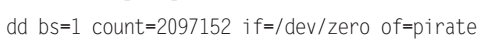
\includegraphics[scale=0.6]{images/lec05-pic01.png}
\end{figure}
Блок в 1024 байт:
\begin{figure}[h]
\centering
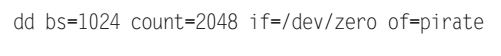
\includegraphics[scale=0.6]{images/lec05-pic02.png}
\end{figure}
\end{block}
\end{frame}

\begin{frame}{Ввод-вывод с пользовательским буфером}
\begin{figure}[h]
\centering
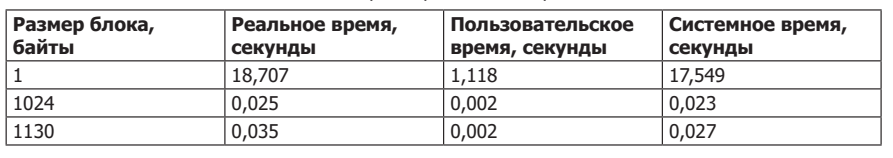
\includegraphics[scale=0.5]{images/lec05-pic03.png}
\end{figure}
\begin{itemize}
\item yа практике размер блока обычно составляет 512, 1024, 2048, 4096 или 8192 байт;
\item для значительного повышения производительности достаточно просто выполнять операции фрагментами, которые являются целочисленными кратными или делителями размера блока;
\item узнать размер блока на конкретном устройстве: системный вызов stat() или  команда stat(1).  
\end{itemize}
\end{frame}

\begin{frame}{Принцип работы пользовательского буфера}
Запись данных:
\begin{itemize}
\item по мере того как данные записываются, они сохраняются в буфере в пределах адресного пространства конкретной программы;
\item когда размер буфера достигает установленного предела, называемого размером буфера, содержимое этого буфера переносится на диск за одну операцию записи. 
\end{itemize}
Считывание данных:
\begin{itemize}
\item поступающие от приложения запросы на считывание имеют разные размеры и обслуживаются не из файловой системы напрямую, а удовлетворяются фрагментами,
получаемыми через буфер;
\item по мере того как приложение считывает все больше и больше информации, данные выдаются из буфера кусками;
\item как только буфер пустеет, начинается считывание следующего сравнительно крупного фрагмента, выровненного по границам блоков. 
\end{itemize}
\end{frame}

\end{document}
